\chapter{Hardware}

Die Hardware besteht aus einem Raspberry Pi, \todo{genauere Beschreibung}
\section{Der Raspberry Pi}
Der \textit{Raspberry Pi} ist ein Einplatinencomputer, der 2012 von der \textit{Raspberry Pi Foundation} auf den Markt gebracht wurde.

\begin{figure}[h]
  \centering
     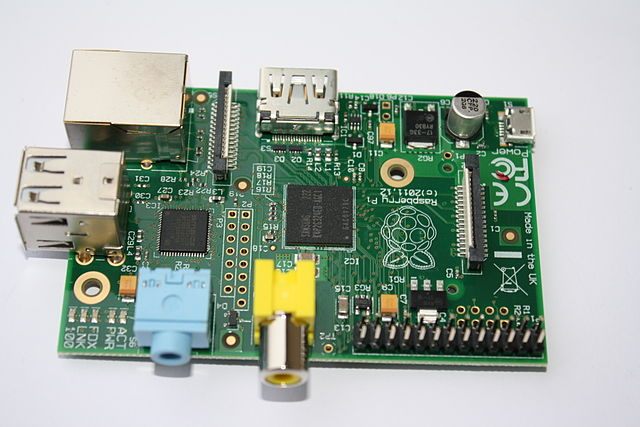
\includegraphics[width=0.8\textwidth]{figures/raspberry.jpg}
 \caption[Raspberry Pi - Modell B]{Raspberry Pi - Modell B\footnotemark}
  \label{fig:raspberry}
\end{figure}
\footnotetext{\cite{rasp_bild}}

\subsection{Geschichte}
Ursprünglich war er als günstiger Computer gedacht, um britischen Jugendlichen das Programmieren näher zu bringen. An der \textit{University of Cambridge} stellte man fest, dass die Vorkenntnisse von Studienanfängern immer geringer wurden, weil sie -- sowohl privat als auch in der Schule -- sich immer weniger mit der Funktionsweise von Computern und Programmen beschäftigen. Daher wollte man einen Computer entwickeln, mit dem die Jugendlichen experimentieren können.
\footcite{aboutraspberry}$^,$
\footcite[Geschichte]{wiki:raspberry}

\subsection{Technische Daten}
Die Technik in einem Raspberry Pi ist vergleichbar mit der eines Smartphones. Der Raspberry Pi hat eine \acrshort{cpu} mit 700 MHz, welche auf bis zu 1 GHz übertaktbar ist, und je nach Modell 256 oder 512 MB Arbeitsspeicher. Als Speichermedium für das Betriebssystem (verschiedene Linux-Distributionen stehen zur Auswahl) wird eine SD-Karte bzw. eine microSD-Karte verwendet.

Zur Stromversorgung genügt ein normales Handy-Ladegerät mit Micro-USB-Anschluss und 1 \gls{Ampere} Stromstärke, denn der Raspberry Pi benötigt nur 3,5 Watt\footcite{strom} (Modell B).

Zum Anschließen anderer Hardware gibt es zwei USB-Anschlüsse und 26 \gls{gpio}-Pins.

\section{Sensoren}
\label{sec:Sensoren}

Zur Messung der Werte werden folgende Sensoren verwendet:
\begin{itemize}
\item 4 Temperatursensoren \textit{DS18B20} (\ref{subsec:Temperatur})
\item Luftfeuchtesensor \textit{DHT22} (\ref{subsec:Luftfeuchtigkeit})
\item Luftdrucksensor \textit{BMP085} (\ref{subsec:Luftdruck})
\item Luftqualitätssensor \textit{VOLTCRAFT CO-20} (\ref{subsec:Luftqualitat})
\item CPU-Temperatur des Raspberry Pi
\end{itemize}
\subsection{Temperatur}
\label{subsec:Temperatur}

%\begin{figure}
%  \centering
%     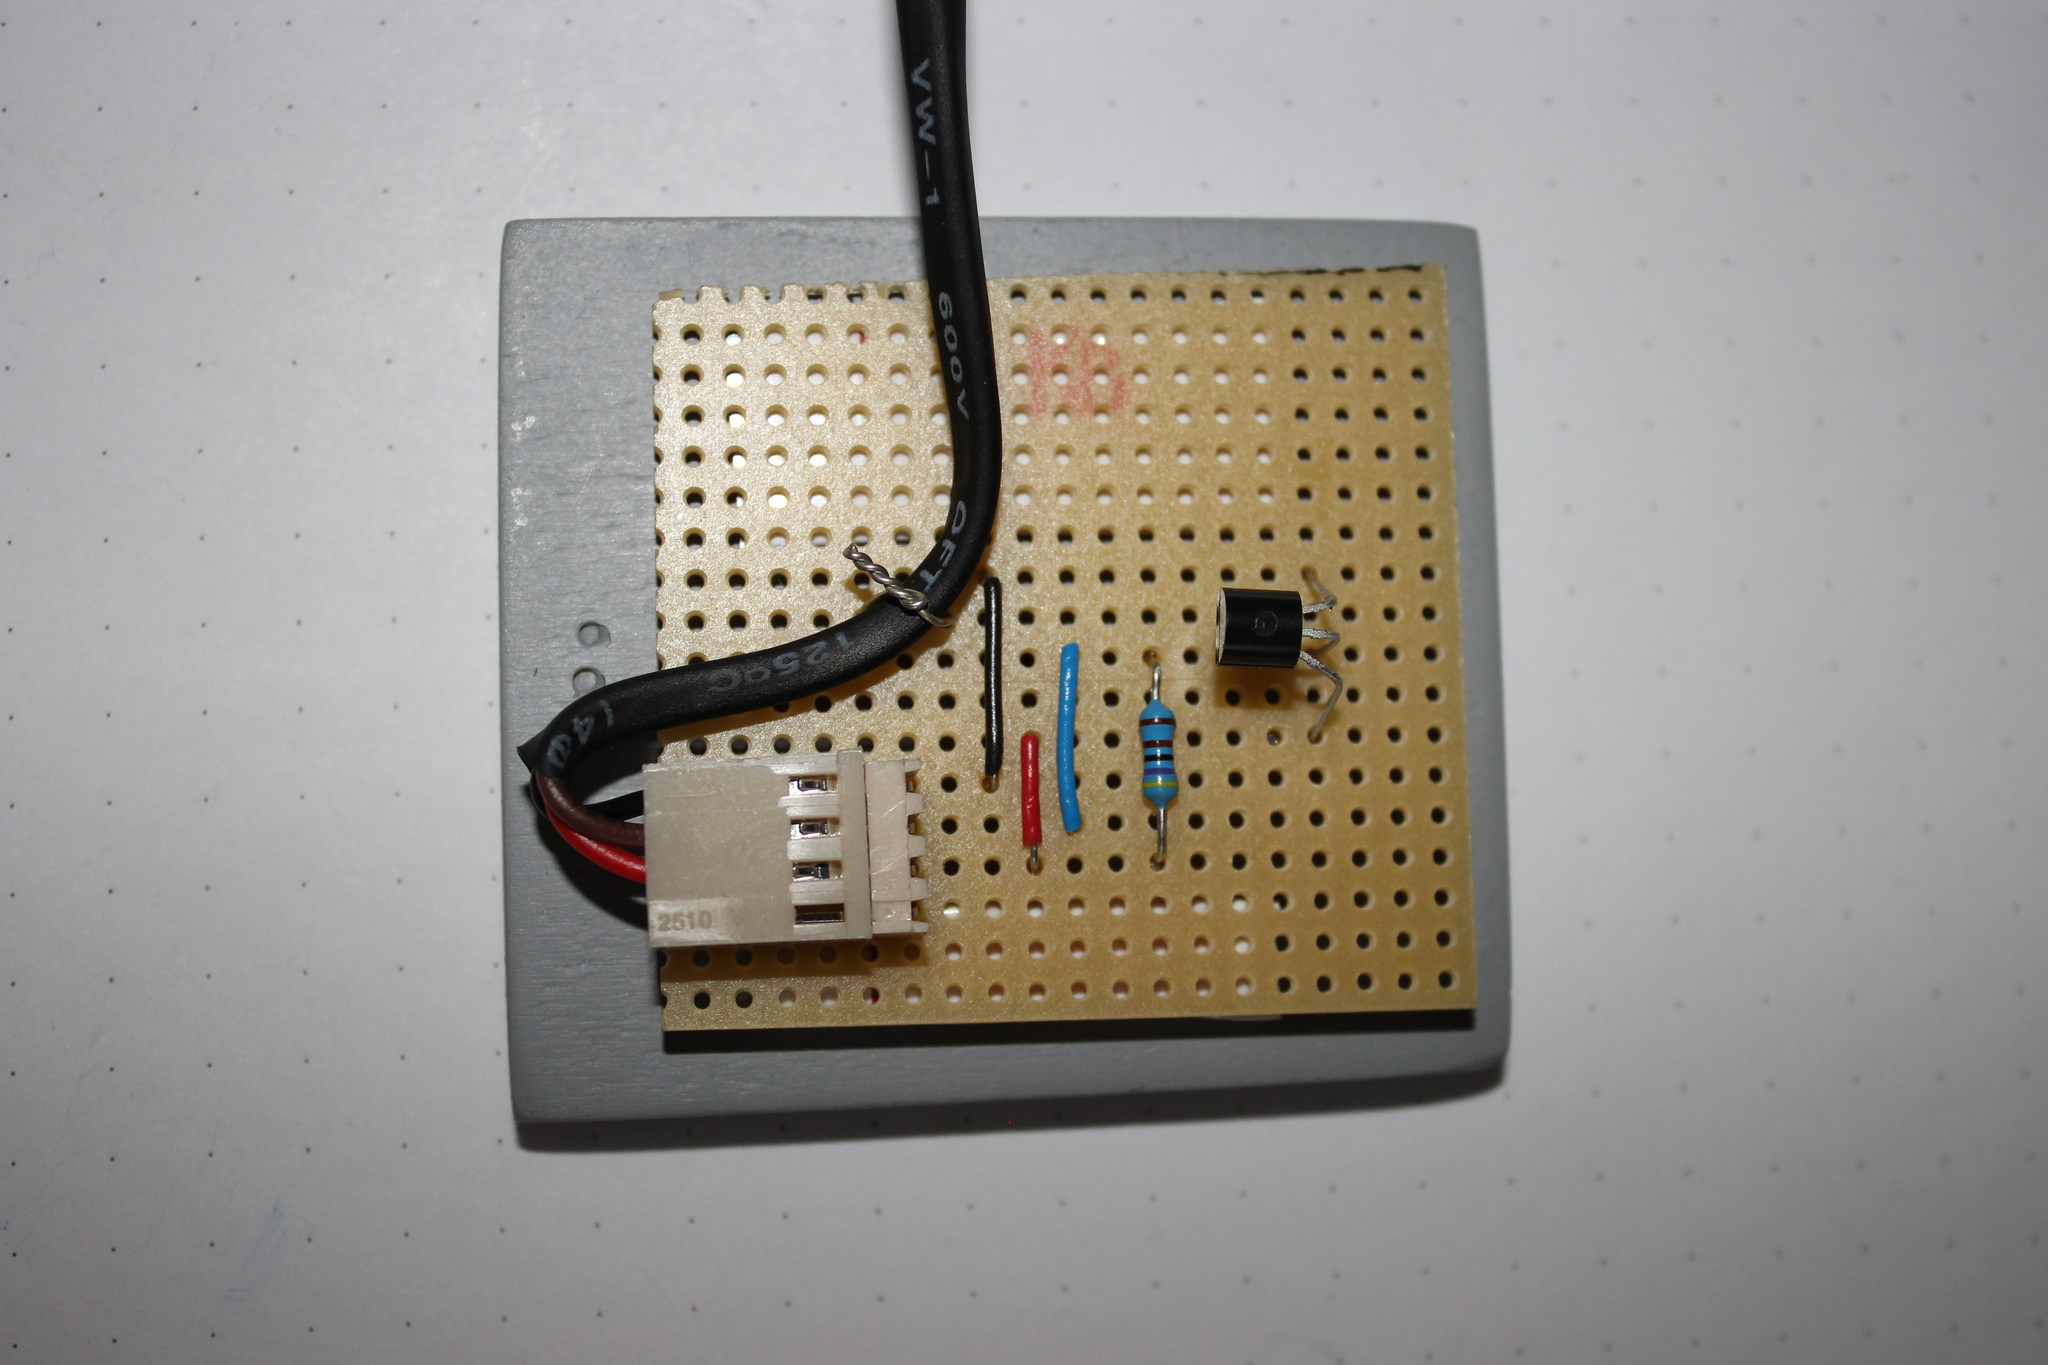
\includegraphics[width=0.4\textwidth]{figures/temp_sensor.jpg}
%  \caption{Platine mit dem DS18B20 für den Innensensor (eigenes Werk)}
%  \label{fig:temp_sensor}
%\end{figure}


Mithilfe der Temperatur"-sensoren werden die Innen"-temperatur, die Gehäuse"-temperatur und die Bodentemperatur (Außen) gemessen. Diese haben eine Messgenauigkeit von \SI{\pm 0.5}{\degreeCelsius}  und einen Messbereich von \SI{-10}{\degreeCelsius}  bis \SI{+85}{\degreeCelsius}. \footcite[20]{temp}

Der Sensor wird mithilfe von einem 1-Wire-Bus ausgelesen. Hierbei benötigt man (außer für die Stromversorgung mit 5 \gls{Volt}) nur ein Kabel, auf dem die Daten übertragen werden.\footcite{1-wire}
Ein weiterer Vorteil von 1-Wire ist, dass nahezu beliebig viele Sensoren auf einem Datenkabel parallel geschaltet werden können. (Abb. \ref{fig:temp_pin})

Die Messdaten des \textit{DS18B20} können auf dem Raspberry Pi sehr einfach ausgelesen werden, weil dies von einem Linux-\gls{Kernelmodul} erledigt wird. Um die Temperatur zu erhalten, muss  nur eine virtuelle Datei ausgelesen werden, welche das Messergebnis in tausendstel Grad Celsius enthält. (Siehe Abbildung \ref{fig:temp_screenshot})
\begin{figure}
  \centering
     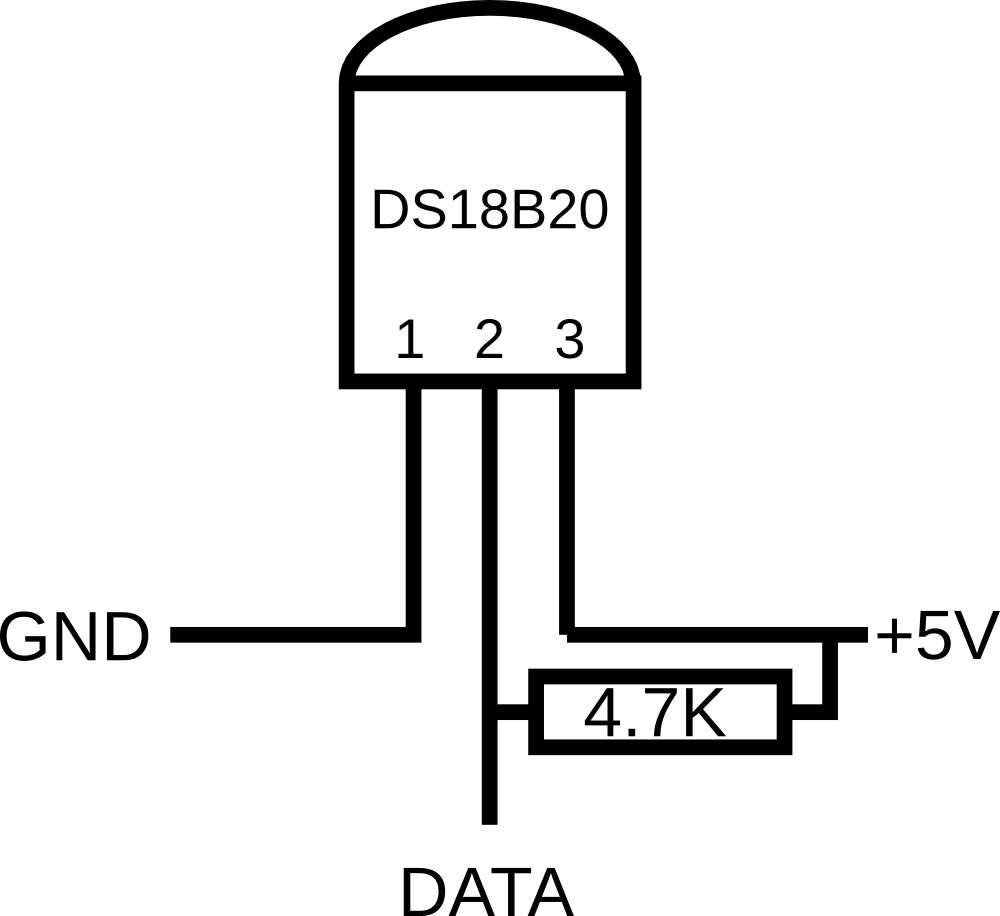
\includegraphics[width=0.4\textwidth]{figures/temp_pin.png}
  \caption{Pinbelegung des DS18B20 (eigenes Werk)}
  \label{fig:temp_pin}
\end{figure}
\begin{figure}[h]
  \centering
     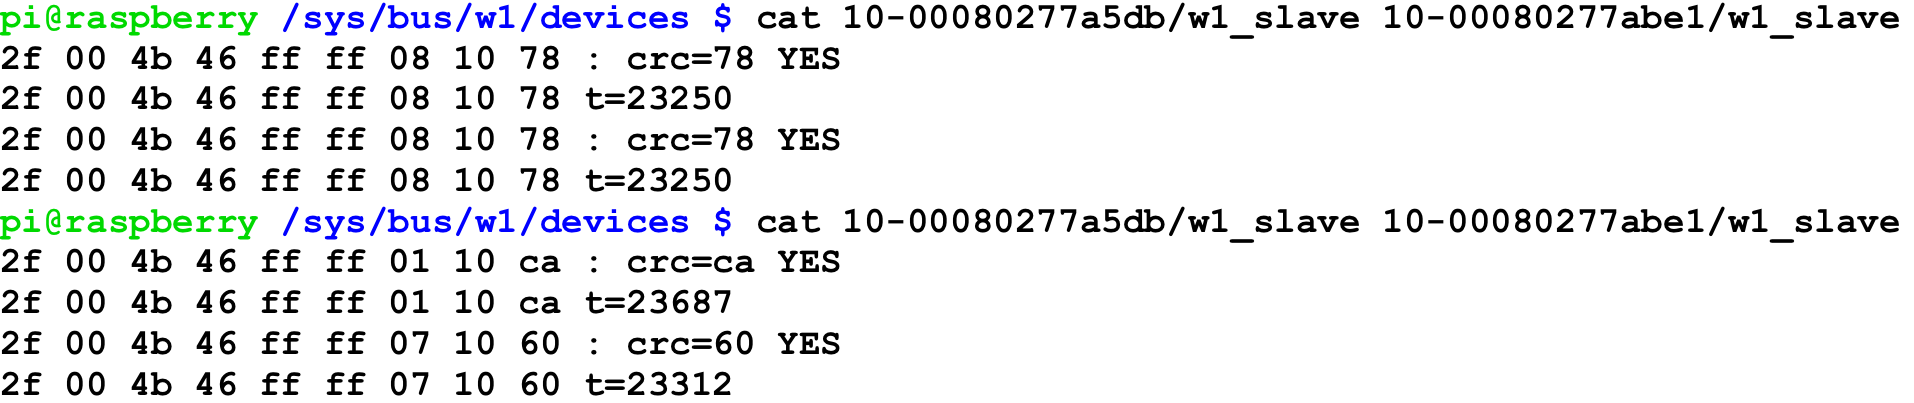
\includegraphics[width=\textwidth]{figures/temp_screenshot.png}
  \caption{Die erste erfolgreiche Messung (eigenes Werk)}
  \label{fig:temp_screenshot}
\end{figure}

\subsection{Luftfeuchtigkeit}
\label{subsec:Luftfeuchtigkeit}

Zum Messen der Luftfeuchtigkeit der Außenluft wird der \textit{DHT22} verwendet. Dieser kann auch die Temperatur messen. Die Messgenauigkeit beträgt \SI{\pm 0.5}{\degreeCelsius} und \SI{\pm 2}{\% .relative.Luftfeuchte}.\footcite{DHT22}
Wie der \textit{DS18B20} (\ref{subsec:Temperatur}) benötigt der Luftfeuchtigkeitssensor zusätzlich zur Stromversorgung nur ein Kabel zur Datenübertragung. Es können jedoch nicht mehrere Sensoren parallel geschaltet werden. \footcite[Wiring]{DHT}

\begin{figure}[h]
  \centering
     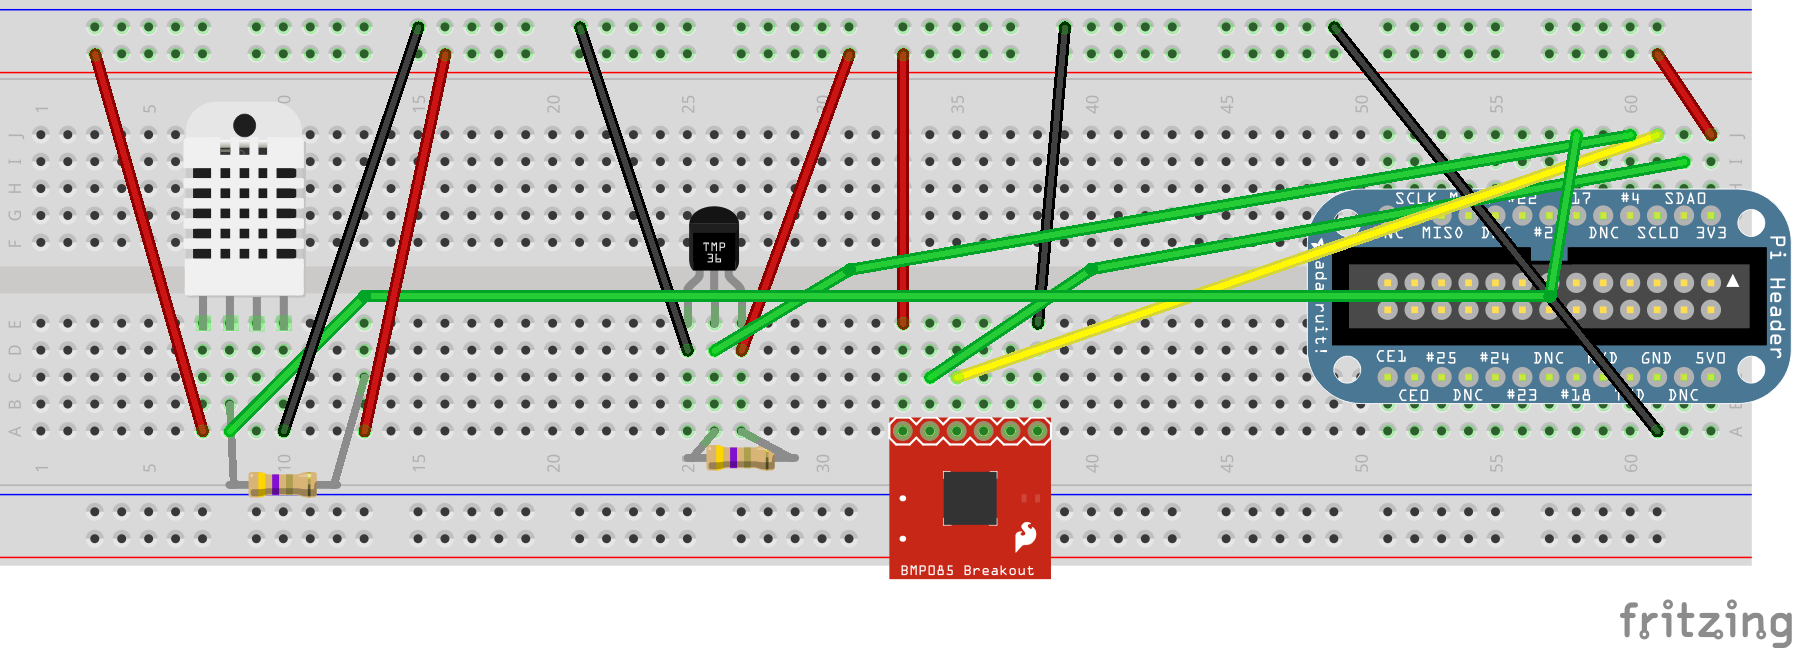
\includegraphics[width=\textwidth]{figures/steckbrett.png}
  \caption{Anschlussskitze von \textit{DS18B20} (Mitte; \ref{subsec:Temperatur}), \textit{DHT22} (Links; \ref{subsec:Luftfeuchtigkeit}) und \textit{BMP085} (Rechts; \ref{subsec:Luftdruck}) (eigenes Werk)}
  \label{fig:steckbrett}
\end{figure}

Die Daten des Sensors werden von einem \gls{C} Programm von Adafruit ausgelesen.
\footcite[Software Install]{DHT}

\subsection{Luftdruck}
\label{subsec:Luftdruck}

Der \textit{BMP085} ist der präziseste Sensor. Er wird zum Messen des Luftdruckes und der Außentemperatur verwendet und hat dabei eine Genauigkeit von\SI{\pm 1.0}{\hecto\pascal} und \SI{0.5}{\degreeCelsius} bei \SI{25}{\degreeCelsius}\footcite[6]{BMP085}

Die Messdaten überträgt der Sensor über einen \gls{I2C}-Bus. Dabei werden (zusätzlich zur Stromversorgung) \textbf{zwei} Kabel zur Datenübertragung benötigt. (siehe Abbildung \ref{fig:steckbrett})
Zum einen ist das das gelbe Kabel, über welches der Raspberry Pi dem Sensor die Taktfrequenz schickt, in der er die Daten übertragen soll, und das grüne Kabel, über das die eigentlichen Daten übertragen werden.
\footcite[Hooking Everything Up]{bmp058_adafruit}

Auch dies wird von einem Programm von Adafruit übernommen. \footcite[Using the Adafruit BMP Python Library (Updated)]{bmp058_adafruit}

\subsection{Luftqualität}
\label{subsec:Luftqualitat}
Der letzte Sensor der hinzugekommen ist, war der \textit{VOLTCRAFT CO-20}. Da reguläre CO\textsubscript{2}-Sensoren teuer sind, habe ich mich für einen einfacheren \acrshort{voc}-Sensor entschieden. Dieser misst die Menge an Flüchtige organischen Verbindungen in der Luft und gibt dafür einen Wert an, der die relative Verschlechterung seit dem Einschalten angibt. Da der \textit{VOLTCRAFT CO-20} jedoch nicht mehr erhältlich ist, verwende ich den baugleichen \enquote{Raumluftfühler} von Velux.\footcite{Velux}

\begin{figure}[h]
  \centering
     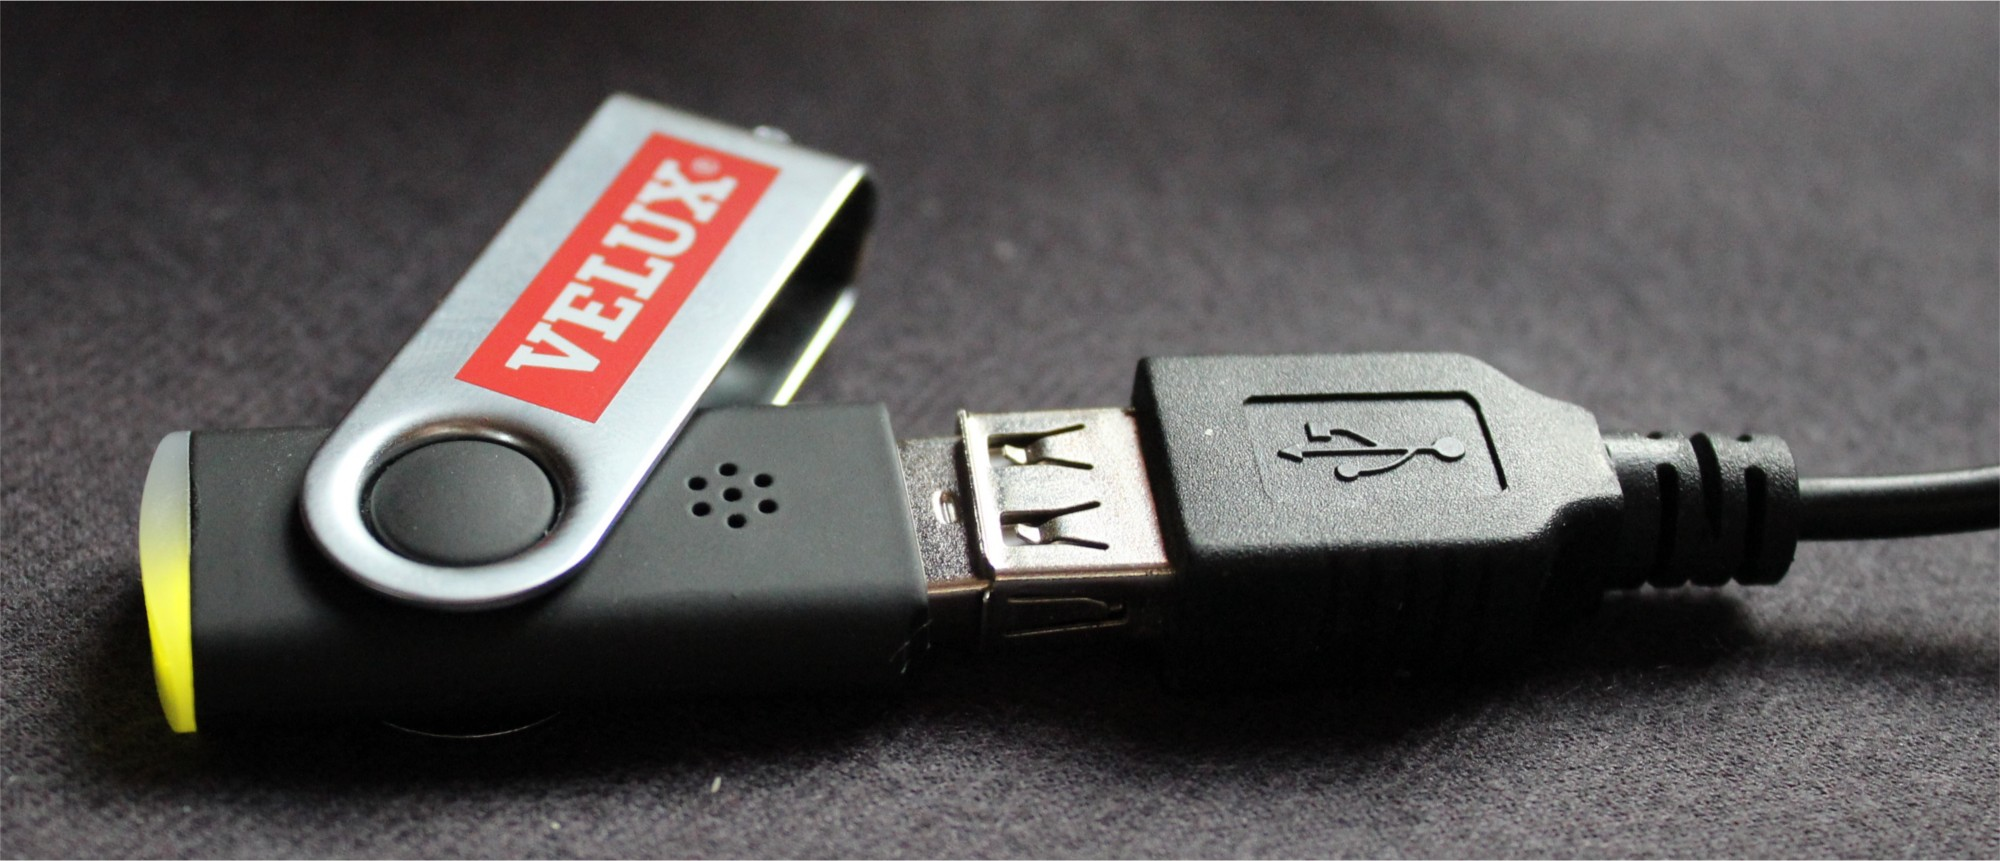
\includegraphics[width=\textwidth]{figures/velux.jpg}
  \caption{Velux-Raumluftfühler}
  \label{fig:velux}
\end{figure}

Der Sensor wird über USB an den Raspberry Pi angeschlossen. Um die Daten unter Linux auszulesen, wird \enquote{usb-sensors-linux} verwendet.\footcite{usb-sensors-linux}
Dies gibt anschließend einen Wert aus, wobei 400 \todo{wirklich 400?} die anfängliche Qualität ist und ein höherer Wert eine schlechtere Luftqualität anzeigt.

\section{Display}
\section{Anschluss}
